\documentclass[usenames, xcolor=dvipsnames]{beamer}
%% \documentclass[professionalfonts, xcolor=table, handout]{beamer}
%% \usepackage{pgfpages}
%% \pgfpagesuselayout{4 on 1}[a4paper,border shrink=5mm, landscape]
\usepackage{fontspec}
\usepackage{amsmath,amssymb}
\usepackage{pifont}% http://ctan.org/pkg/pifont
\usepackage{tikz}
\usetikzlibrary{positioning, matrix, arrows.meta, shapes.geometric, calc,
  decorations.pathmorphing, decorations.pathreplacing, fit, shapes.multipart}
\usepackage{mathabx}
\usepackage{mathtools}
\usepackage{mathpartir}
\usepackage{fancyvrb}
\usepackage{stmaryrd}
\usepackage[absolute,overlay]{textpos}
\usepackage[export]{adjustbox} % for subfigures

\definecolor{lightg}{RGB}{217,232,225}
\definecolor{darkg}{RGB}{6,81,42}
\definecolor{myred}{rgb}{0.0, 0.42, 0.24}
\colorlet{mypink}{myred!50!white}
\definecolor{mymaroon}{rgb}{0.86, 0.08, 0.24}

\defaultfontfeatures{Mapping=tex-text,Scale=MatchLowercase}
% \setmainfont{Libertinus Serif}
% \setsansfont{Libertinus Sans}
% \setmonofont{Menlo Regular}
\usetheme{Madrid}
\useoutertheme{infolines} % Alternatively: miniframes, infolines, split
\useinnertheme{circles}

% \setbeamertemplate{enumerate item}[default]
\usecolortheme[named=myred]{structure}
% \usecolortheme{spruce}
\usefonttheme{serif}
\setbeamerfont*{frametitle}{series=\bfseries}
\setbeamercolor{alerted text}{fg=mymaroon}
\setbeamertemplate{navigation symbols}{}
\setbeamercolor{emphC}{fg=myred}
% \setbeamercolor{block title}{bg = darkg, fg=white!80}
% \setbeamercolor{block body}{bg = lightg, fg=black}
\setbeamercolor{itemize item}{fg=black}
\setbeamercolor{description item}{fg=myred}

\newcommand{\sz}{\texttt{SIZE}}
\newcommand{\ifty}{\texttt{INF}}
\newcommand{\scon}{\mathbin{\ast}}
\usepackage{scalerel}
\renewcommand{\bigstar}{\raisebox{-0.24em}{{\scaleobj{2.5}{\scon}}}}

\newcommand{\ocon}{%
  \mathbin{\mbox{$\mathrlap{\cup}\hspace*{.15em}
      \raisebox{.01em}[0ex][0ex]{$\scon$}$\hspace*{.07em}}}}
\newcommand{\medocon}{
  \raisebox{-0.3ex}{\resizebox{0.63em}{!}{$\scon$}} \hspace{-2.4ex} \bigcup}
\newcommand{\wand}{%
 \mathrel{\mbox{$\hspace*{-0.03em}\mathord{-}\hspace*{-0.66em}
  \mathord{-}\hspace*{-0.36em}\mathord{\scon}$\hspace*{-0.005em}}}}
\newcommand{\defeq}{\mathbin{\overset{\mathrm{def}}{=}}}
\newcommand{\emphd}[1]{{\bfseries #1}}
\newcommand{\emphr}[2]{\alert<#1>{#2}}
\newcommand{\bracket}[1]{[#1]}
\newcommand{\hide}[1]{}
\newcommand{\braces}[1]{\left\{\begin{array}{l@{}} #1 \end{array}\right\}}

\makeatletter\let\frametextheight\beamer@frametextheight\makeatother
\newcommand\credit[1]{%
  \begin{textblock*}{\paperwidth}(0pt,\textheight)
    \raggedleft #1\hspace{.5em}
\end{textblock*}}
\newcommand{\pguards}[1]{\llbracket #1 \rrbracket}
\newcommand{\xmark}{\ding{55}}%
\newcommand{\cmark}{\ding{51}}%
\newcommand{\m}[1]{\ensuremath{\mathit{#1}}} % math font
\newcommand{\p}[1]{\ensuremath{\mathsf{#1}}} % predicate font
\newcommand{\bi}{\Leftrightarrow} % equivalence of expressions


\title[Verified Dijkstra in C]{Verified C Implementation of Dijksta's Algorithm}
\author[Mohan, Hobor]{\underline{Anshuman Mohan}, Aquinas Hobor}
\institute[NUS]{
\includegraphics[height=0.12\textwidth]{NUS_logo_full-horizontal.jpg}}
  \date[APLAS SRC 2019]{APLAS Student Research Competition \\ \today}

\begin{document}
\begin{frame}[plain]
  \titlepage
\end{frame}

\begin{frame}{Saluting the Mothership}

\includegraphics[scale=0.09]{vst_logo}
\hspace{2em} 
\includegraphics[scale=0.12]{compcert_logo}
\hspace{2em} 
\includegraphics[scale=0.2]{paper_screen}

\bigskip
VST + CompCert + 25000 \textsc{loc} library

\bigskip
Powerful enough to verify \alert{executable code}
\\\hspace{1em}against \alert{realistic specifications}
\\\hspace{2em}expressed with \alert{mathematical graphs}

\bigskip
\flushright [{\footnotesize Wang \emph{et. al.}}, \textsc{pacmpl oopsla} {\footnotesize 2019}]
\end{frame}

\begin{frame}{This Work}

\includegraphics[scale=0.09]{vst_logo}
\hspace{2em} 
\includegraphics[scale=0.12]{compcert_logo}
\hspace{2em} 
\includegraphics[scale=0.2]{paper_screen}

\bigskip

Never used edge labels... 

\pause

Not unlike vertex labels, but let's try anyway

\pause
\flushright{\alert{Verify Dijkstra's one-to-all shortest path algorithm}}
\end{frame}

\begin{frame}{Challenges}

Using CompCert C 
\\ \hspace{1em} executable and realistic 
\\ \hspace{1em} \alert{real-world complications}

\bigskip

Aiming for \alert{full functional correctness}
\\ \hspace{1em} and not just safety 

\end{frame}

\begin{frame}{Refresher}

\colorlet{stash}{red}
\colorlet{red}{myred}
\begin{center}
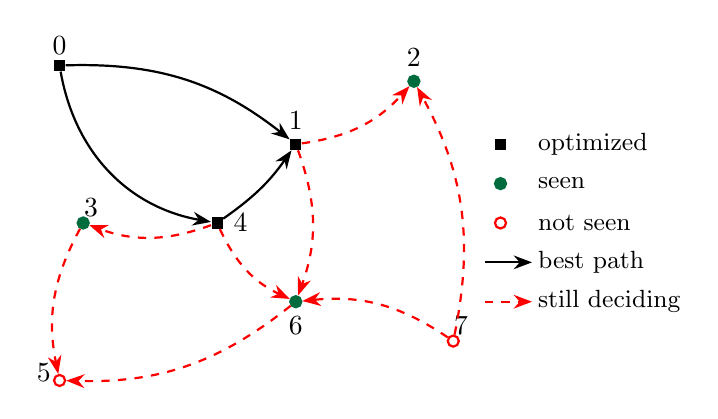
\begin{tikzpicture}
[vad/.style={rectangle, fill=black, inner sep=0pt, minimum size=4pt},
 inf/.style={circle, draw=red, thick, inner sep=0pt, minimum size=4pt},
 inv/.style={circle, fill=myred, draw=myred, thick, inner sep=0pt, minimum size=4pt},
 ->/.style={thick, arrows={-Stealth}}]
\node at (0.3,0) {$4$}; % n1
\node[vad] (n1) at (0, 0) {};
\node at (1, 1.3) {$1$}; % n2
\node[vad] (n2) at (1, 1) {};
\node at (1, -1.3) {$6$}; % n3
\node[inv] (n3) at (1, -1) {}; %
\node at (-2,2.25) {$0$}; % n4
\node[vad] (n4) at (-2,2) {}; 
\node at (-2.2,-1.9) {$5$}; % n5
\node[inf] (n5) at (-2,-2) {};
\node at (-1.6,0.2) {$3$}; % n6
\node[inv] (n6) at (-1.7,0) {};
\node at (2.5,2.1) {$2$}; % n7
\node[inv] (n7) at (2.5,1.8) {};
\node at (3.1,-1.3) {$7$}; % n8
\node[inf] (n8) at (3,-1.5) {};
\draw[->] (n1) to [bend right=10] (n2);
\draw[->, dashed, red] (n1) to [bend right=20] (n3);
\draw[->,dashed,red] (n3) to [bend left=20] (n5);
% \draw[->,dashed,red] (n3) to (n8);
\draw[->,dashed,red] (n2) to [bend left=20] (n3);
\draw[->,dashed,red] (n2) to [bend right=20] (n7);
\draw[->,dashed,red] (n8) to [bend right=20] (n3);
\draw[->,dashed,red] (n8) to [bend right=20] (n7);
% \draw[->] (n4) to [bend left=20] (n1);
% \draw[->, dashed, red] (n1) to [bend right=20] (n5);
\draw[->] (n4) to [bend left=20] (n2);
\draw[->, dashed, red] (n1) to [bend left=20] (n6);
\draw[->, dashed, red] (n6) to [bend right=20] (n5);
\draw[->] (n4) to [bend right=35] (n1);
% \node at (-0.6, 1.7) {$\m{e}$};
% key on the side:
\node[vad] (n9) at (3.6, 1) {};
\node[inv] (n10) at (3.6, 0.5) {};
\node[inf] (n11) at (3.6, 0) {};
\draw[->] (3.4, -0.5) -- (4, -0.5);
\draw[->,dashed,red] (3.4, -1) -- (4, -1);
\node at (3.9, 1) [right=1.5pt] {\small optimized};
\node at (3.9, 0.5) [right=1.5pt] {\small seen};
\node at (3.9, 0) [right=1.5pt] {\small not seen};
\node at (3.9, -0.5) [right=1.5pt] {\small best path};
\node at (3.9, -1) [right=1.5pt] {\small still deciding};


\end{tikzpicture}
\end{center}
\colorlet{red}{stash}

\end{frame}



\begin{frame}{Instantiating DijkGraph}
A PreGraph is a hextuple (\texttt{VType}, \texttt{EType}, \texttt{vvalid}, \texttt{evalid}, \texttt{src}, \texttt{dst})
\vspace{-1.5em}
\begin{flushleft}
\begin{equation*}
\begin{split}
\textbf{Dijk\_PG($\gamma$) $\defeq$ \null} & \texttt{VType := Z} \\
                    &\texttt{EType := VType * VType} \\
                    &\texttt{src := fst} \\
                    &\texttt{dst := snd} \\ 
                    &\forall \m{v}.~\texttt{vvalid}(\gamma, \m{v}) \bi 0 \le \m{v} < {\sz} \\
                    &\forall \m{s,d}.~\texttt{evalid}(\gamma, \m{(s,d)}) \bi \texttt{vvalid}(\gamma, \m{s}) \wedge \texttt{vvalid}(\gamma, \m{d})
\end{split}
\end{equation*}
\end{flushleft}
\end{frame}

\begin{frame}[fragile]{Instantiating DijkGraph}
A LabeledGraph is a quadruple (PreGraph, \texttt{VL}, \texttt{EL}, \texttt{GL})
\vspace{-1.5em}
\begin{flushleft}
\begin{equation*}
\begin{split}
\textbf{Dijk\_LG($\gamma$) $\defeq$ \null} &\text{Dijk\_PG as shown} \\
                  &\texttt{VL := list EL} \\
                  &\texttt{EL := Z} \\
                  &\texttt{GL := unit} 
\end{split}
\end{equation*}
\end{flushleft}
\end{frame}

\begin{frame}[fragile]{Instantiating DijkGraph}
A GeneralGraph adds arbitrary soundness conditions
\vspace{-1.5em}
\begin{flushleft}
\begin{equation*}
\begin{split}
\textbf{DijkGraph($\gamma$) $\defeq$ \null} &\text{Dijk\_LG as shown, and } \\
                    &FiniteGraph(\gamma) \wedge \null \\
                    &\forall \m{i,j}.~\texttt{vvalid}(\gamma, \m{i}) \wedge \texttt{vvalid}(\gamma, \m{j}) \Rightarrow \\
                    &\qquad \m{i} = \m{j} \Rightarrow \texttt{elabel}(\gamma,(\m{i},{j})) = 0 \wedge \null \\
                    &\qquad \m{i} \neq \m{j} \Rightarrow 0 \le \texttt{elabel}(\gamma,(\m{i},{j})) \le \alert<2>{\lfloor \texttt{MAX/SIZE} \rfloor}
\end{split}
\end{equation*}
\end{flushleft}
\end{frame}

\begin{frame}{Representing DijkGraph in Memory}
\begin{equation*}
\begin{split}
\p{list\_rep}(\gamma, \m{i}) &\defeq \texttt{data\_at  array  graph2mat}(\gamma)[\m{i}] \texttt{  list\_addr}(\gamma, \m{i}) \\
\vspace{1em}
\p{graph\_rep}(\gamma) &\defeq \underset{\texttt{vvalid}(\gamma,\m{v})}{\bigstar} \m{v}  \mapsto\p{list\_rep}(\gamma, \m{v})
\end{split}
\end{equation*}

\end{frame}

\begin{frame}[fragile]{Code and Specification}

\begin{Verbatim}[commandchars=\\\{\}]
#define \alert{IFTY INT_MAX - INT_MAX/SIZE}
\end{Verbatim}
\begin{Verbatim}
void dijkstra (int graph[SIZE][SIZE], int src, 
                        int *dist, int *prev) {
\end{Verbatim}
$\braces{\p{DijkGraph}(\gamma)}$
\pause
\begin{Verbatim}
 int pq[SIZE];
 int i, j, u, cost;
 for (i = 0; i < SIZE; i++)
 {  dist[i] = INF; prev[i] = INF; pq[i] = INF;  }
 dist[src] = 0; pq[src] = 0; prev[src] = src;
\end{Verbatim}
\pause
$\braces{\p{DijkGraph}(\gamma) \wedge \alert{\m{dijk\_correct}(\gamma,\m{src},\m{prev},\m{dist},\m{priq})}}$
\begin{Verbatim}
 // big while loop
\end{Verbatim}
\end{frame}

\begin{frame}[fragile]{Code and Specification}
$\braces{\p{DijkGraph}(\gamma) \wedge \m{dijk\_correct}(\gamma,\m{src},\m{prev},\m{dist},\m{priq})}$
\pause
\begin{Verbatim}
 while (!pq_emp(pq)) {
  u = popMin(pq);
  for (i = 0; i < SIZE; i++) {
   cost = graph[u][i]; 
    if (cost < INF) {
     if (dist[i] > dist[u] + cost) {
      dist[i] = dist[u] + cost; prev[i] = u; pq[i] = dist[i];
 }}}}
\end{Verbatim}
\pause
$\braces{\p{DijkGraph}(\gamma) \wedge 
\alert{\forall \m{dst} \in \m{priq}.~\m{priq}[\m{dst}] = \texttt{INF}} \wedge \null \\ 
\m{dijk\_correct}(\gamma,\m{src},\m{prev},\m{dist},\m{priq})}$
\begin{Verbatim}
return;
}
\end{Verbatim}
\end{frame}

\begin{frame}{Dijkstra\_Correct}

\begin{equation*}
\begin{split}
\m{dijk\_correct}(\gamma, \m{src}, \m{prev}, \m{dist},& \m{priq}) \; \defeq \; \\
\alert<2>{\forall \m{dst}.~\m{dst} \in \m{popped}(\m{priq}) \; \Rightarrow} \; & \\ 
& \hspace{-5em} \exists \m{path}.~\m{path\_correct}(\gamma, \m{prev}, \m{dist}, \m{path}) \wedge \null \\
& \hspace{-5em} \m{path\_glob\_optimal}(\gamma, \m{dist}, \m{path}) \wedge \null \\
& \hspace{-5em} \m{path\_entirely\_in\_popped}(\gamma, \m{prev}, \m{path}) \wedge \null \\
\alert<3>{\m{priq}[\m{dst}] < \ifty \; \Rightarrow} \; & \\ 
& \hspace{-5em} \texttt{let }\m{m} \texttt{ := } \m{prev}[\m{dst}] \texttt{ in } \m{m} \in \m{popped}(\m{priq}) \wedge \null \\
& \hspace{-5em} \forall \m{m'} \in \m{popped}(\m{priq}).~\m{cost}(\m{path2m} +:: (m, dst)) \le \null \\
& \hspace{-5em} \hspace{10em} \m{cost}(\m{path2m'} +:: (m', dst)) \wedge \null \\
\alert<4>{\m{priq}[\m{dst}] = \ifty \; \Rightarrow} \; & \\ 
& \hspace{-5em} \forall \m{m} \in \m{popped}(\m{priq}).~\m{cost}(\m{path2m} +:: (m, dst)) = \ifty
\end{split}
\end{equation*}

\end{frame}

\newcommand{\s}{11}
\begin{frame}{Key Transformation: Growing the Subgraph}

\begin{center}
\begin{adjustbox}{scale=0.50}
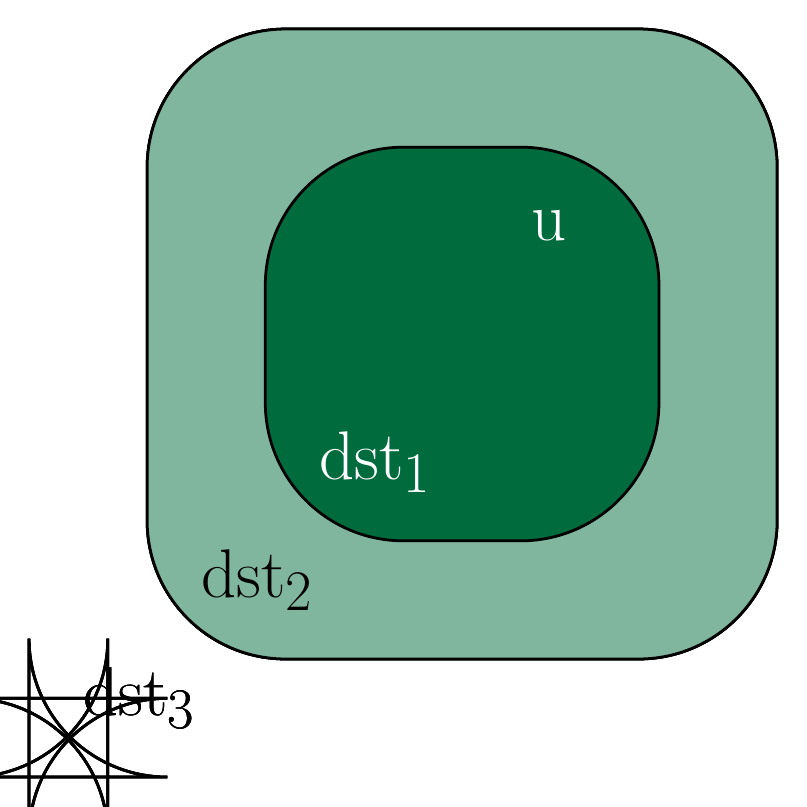
\begin{tikzpicture}[on grid,
  popped/.style={rounded corners=50pt, line width=1pt, draw, fill=myred},
  fringe/.style={rounded corners=50pt, line width=1pt, draw, fill=mypink},
  popping/.style={rounded corners=50pt, line width=1pt, draw, dashed, fill=mymaroon},
  unseen/.style={rounded corners=50pt, line width=1pt, draw}]
  \uncover<1>{
  \draw[unseen] (0,0) -- (\s,0) -- (\s,\s) -- (0,\s) -- cycle;
  \draw[fringe] (1.5,1.5) -- (9.5,1.5) -- (9.5,9.5) -- (1.5,9.5) -- cycle;
  \draw[popped] (3,3) -- (8,3) -- (6,6) -- (3,8) -- cycle;
  \node at (1.4,1) {\Huge dst$_3$};   
  \node at (2.9,2.5) {\Huge dst$_2$};   
  \node at (4.4,4) {\Huge \color{white}dst$_1$}; 
  \node at (6.6,7) {\Huge u};}
  \uncover<2>{
    \draw[unseen] (0,0) -- (\s,0) -- (\s,\s) -- (0,\s) -- cycle;
  \draw[fringe] (1.5,1.5) -- (9.5,1.5) -- (9.5,9.5) -- (1.5,9.5) -- cycle;
  \draw[popping] (3,3) -- (8,3) -- (8,8) -- (3,8) -- cycle;
  \draw[popped] (3,3) -- (8,3) -- (6,6) -- (3,8) -- cycle;
  \node at (1.4,1) {\Huge dst$_3$};   
  \node at (2.9,2.5) {\Huge dst$_2$};   
  \node at (4.4,4) {\Huge \color{white}dst$_1$}; 
  \node at (6.6,7) {\Huge u}; }
  \uncover<3>{
    \draw[unseen] (0,0) -- (\s,0) -- (\s,\s) -- (0,\s) -- cycle;
  \draw[fringe] (1.5,1.5) -- (9.5,1.5) -- (9.5,9.5) -- (1.5,9.5) -- cycle;
  \draw[popped] (3,3) -- (8,3) -- (8,8) -- (3,8) -- cycle;
  \node at (1.4,1) {\Huge dst$_3$};   
  \node at (2.9,2.5) {\Huge dst$_2$};   
  \node at (4.4,4) {\Huge \color{white}dst$_1$}; 
  \node at (6.6,7) {\Huge \color{white}u}; }
\end{tikzpicture}
\end{adjustbox}
\end{center}
\end{frame}

\begin{frame}{Overflow Strikes Again}

The longest optimal path has \texttt{SIZE-1} links \\
\hspace{1em} \pause so say we set \texttt{elabel}'s upper bound to $\lfloor\texttt{MAX/(SIZE-1)}\rfloor$ 

\bigskip \pause
\texttt{MAX} = 7, \texttt{SIZE} = 3, so $0 \le \texttt{elabel}(\gamma, \m{e}) \le 3$.

\bigskip

{\centering
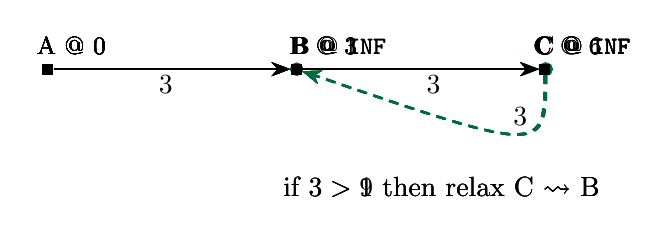
\begin{tikzpicture}
[vad/.style={rectangle, fill=black, inner sep=0pt, minimum size=4pt},
 inf/.style={circle, draw=myred, thick, inner sep=0pt, minimum size=4pt},
 inv/.style={circle, fill=myred, draw=myred, thick, inner sep=0pt, minimum size=4pt},
 ->/.style={thick, arrows={-Stealth}}]

  \node at (1.5,-0.2) {3};
  \node at (4.9,-0.2) {3};
  \node at (6,-0.6) {3};


\uncover<3>{
\node at (0.3, 0.3) {\small A @ 0};
\node at (3.7, 0.3) {\small B @ \ifty};
\node at (6.8, 0.3) {\small C @ \ifty}; 
  \node[vad] (A) at (0,0) {};
  \node[inf] (B) [right = 3 of A] {};
  \node[inf] (C) [right = 3 of B] {};
  \draw [->, dashed, myred] (A) -- (B);
  \draw [->, dashed, myred] (B) -- (C);
  \draw [->, dashed, myred] (C.south) .. controls ++(0, -1) .. (B);}
 
\uncover<4>{
\node at (0.3, 0.3) {\small A @ 0};
\node at (3.7, 0.3) {\small B @ \ifty};
\node at (6.8, 0.3) {\small C @ \ifty};  
  \node[vad] (A) at (0,0) {};
  \node[inv] (B) [right = 3 of A] {};
  \node[inf] (C) [right = 3 of B] {};
  \draw [->, dashed, myred] (A) -- (B);
  \draw [->, dashed, myred] (B) -- (C);
  \draw [->, dashed, myred] (C.south) .. controls ++(0, -1) .. (B);}

\uncover<5>{
\node at (0.3, 0.3) {\small A @ 0};
\node at (3.5, 0.3) {\small B @ 3};
\node at (6.8, 0.3) {\small C @ \ifty};  
  \node[vad] (A) at (0,0) {};
  \node[vad] (B) [right = 3 of A] {};
  \node[inf] (C) [right = 3 of B] {};
  \draw [->] (A) -- (B);
  \draw [->, dashed, myred] (B) -- (C);
  \draw [->, dashed, myred] (C.south) .. controls ++(0, -1) .. (B);
  }

\uncover<6>{ 
\node at (0.3, 0.3) {\small A @ 0};
\node at (3.5, 0.3) {\small B @ 3};
\node at (6.8, 0.3) {\small C @ \ifty};  
  \node[vad] (A) at (0,0) {};
  \node[vad] (B) [right = 3 of A] {};
  \node[inv] (C) [right = 3 of B] {};
  \draw [->] (A) -- (B);
  \draw [->, dashed, myred] (B) -- (C);
  \draw [->, dashed, myred] (C.south) .. controls ++(0, -1) .. (B);
}

\uncover<7>{ 
\node at (0.3, 0.3) {\small A @ 0};
\node at (3.5, 0.3) {\small B @ 3};
\node at (6.6, 0.3) {\small C @ 6};  
  \node[vad] (A) at (0,0) {};
  \node[vad] (B) [right = 3 of A] {};
  \node[vad] (C) [right = 3 of B] {};
  \draw [->] (A) -- (B);
  \draw [->] (B) -- (C);
  \draw [->, dashed, myred] (C.south) .. controls ++(0, -1) .. (B);
}

\uncover<8>{ 
\node at (0.3, 0.3) {\small A @ 0};
\node at (3.5, 0.3) {\small B @ 3};
\node at (6.6, 0.3) {\small C @ 6};  
\node at (5, -1.5) {if $3 > 9$ then relax C $\leadsto$ B};
  \node[vad] (A) at (0,0) {};
  \node[vad] (B) [right = 3 of A] {};
  \node[vad] (C) [right = 3 of B] {};
  \draw [->] (A) -- (B);
  \draw [->] (B) -- (C);
  \draw [->, dashed, myred] (C.south) .. controls ++(0, -1) .. (B);
}

\uncover<9>{ 
\node at (0.3, 0.3) {\small A @ 0};
\node at (3.5, 0.3) {\small B @ 3};
\node at (6.6, 0.3) {\small C @ 6};  
\node at (5, -1.5) {if $3 > \alert{1}$ then relax C $\leadsto$ B};
  \node[vad] (A) at (0,0) {};
  \node[vad] (B) [right = 3 of A] {};
  \node[vad] (C) [right = 3 of B] {};
  \draw [->] (A) -- (B);
  \draw [->] (B) -- (C);
  \draw [->, dashed, myred] (C.south) .. controls ++(0, -1) .. (B);
}

\uncover<10->{ 
\node at (0.3, 0.3) {\small A @ 0};
\node at (3.5, 0.3) {\small B @ \alert{1}};
\node at (6.6, 0.3) {\small C @ 6}; 
\node at (5, -1.5) {if $3 > 1$ then \alert{relax C $\leadsto$ B}};
  \node[vad] (A) at (0,0) {};
  \node[vad] (B) [right = 3 of A] {};
  \node[vad] (C) [right = 3 of B] {};
  \draw [->] (A) -- (B);
  \draw [->] (B) -- (C);
  \draw [->, dashed, myred] (C.south) .. controls ++(0, -1) .. (B);
}

\end{tikzpicture}

}

\bigskip

\uncover<11->{
One solution: Conservatively set upper bound to $\lfloor\texttt{MAX/SIZE}\rfloor$}

\bigskip

\uncover<12->{
Max path cost is then  
$\lfloor\texttt{MAX/SIZE}\rfloor$ \texttt{ * (SIZE-1) = \alert{MAX - }} \alert{$\lfloor\texttt{MAX/SIZE}\rfloor$}}
\end{frame}

\begin{frame}{Overflow Strikes Again}

There are other ways to fix this!
\\ \pause \hspace{1em} \alert{Refactor} troublesome addition as subtraction
\\ \pause \hspace{1em} \alert{Never look back} into optimized part
\\ \pause \hspace{1em} Your suggestion here
\\ \pause \hspace{1em} Your suggestion here

\bigskip

\pause That is not the point
\\ \pause \hspace{1em} \alert{Intuition supports \texttt{INF = MAX}}
\\ \pause \hspace{1em} No reason to do any of the above\pause... until today

\end{frame}


\hide {
\begin{frame}{Recap: Intuitive Specification}
\emph{Primum non nocere}: first, do no harm

\bigskip

\begin{center}
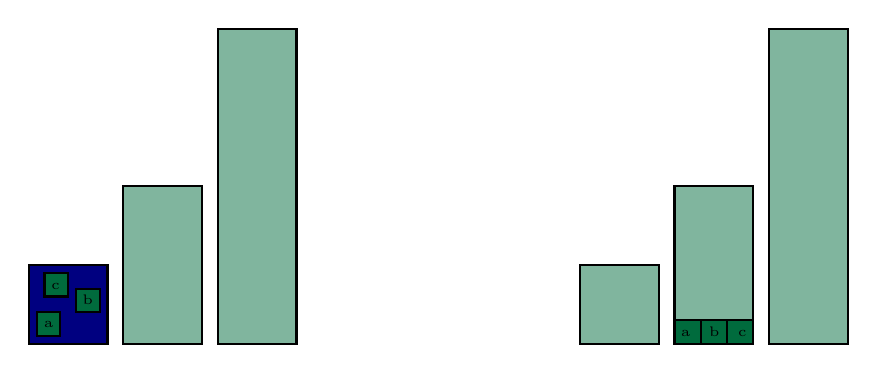
\begin{tikzpicture}
\uncover<1>{
            \draw [fill=NavyBlue, thick]
  (0,0) -- (1,0) -- (1,1) -- (0,1) -- cycle;
            \draw [fill=myred, thick]
  (0.1,0.1) -- (0.4,0.1) -- (0.4,0.4) -- (0.1,0.4) -- cycle;
            \draw [fill=myred, thick]
  (0.6,0.4) -- (0.9,0.4) -- (0.9,0.7) -- (0.6,0.7) -- cycle;
            \draw [fill=myred, thick]
  (0.2,0.6) -- (0.5,0.6) -- (0.5,0.9) -- (0.2,0.9) -- cycle;
            \draw [fill=mypink, thick ] 
  (1.2,0) -- (2.2,0) -- (2.2,2) -- (1.2,2) -- cycle;
            \draw [fill=mypink, thick ] 
  (2.4,0) -- (3.4,0) -- (3.4,4) -- (2.4,4) -- cycle;}

\node at (0.25,0.25){\tiny a};
\node at (0.75,0.56){\tiny b};
\node at (0.34,0.73){\tiny c};

\tikzset{shift={(7,0)}}
  \uncover<1>{
            \draw [fill=mypink, thick ]
  (0,0) -- (1,0) -- (1,1) -- (0,1) -- cycle;
            \draw [fill=mypink, thick ] 
  (1.2,0) -- (2.2,0) -- (2.2,2) -- (1.2,2) -- cycle;
            \draw [fill=mypink, thick ] 
  (2.4,0) -- (3.4,0) -- (3.4,4) -- (2.4,4) -- cycle;
  \draw [fill=myred, thick]
  (1.2,0) -- (2.2,0) -- (2.2,0.3) -- (1.2,0.3) -- cycle;
  \draw[thick] (1.533,0) -- (1.533,0.3);
  \draw[thick] (1.866,0) -- (1.866,0.3);
  \node at (1.7,0.15){{\tiny a} \hspace{0.01em} {\tiny b} \hspace{0.01em} {\tiny c}};}
  \end{tikzpicture}
\end{center}

\uncover<1>{\vspace{-6em}\hspace{5.8cm}\Huge $\cong$}
\end{frame}

\section{Findings}

\begin{frame}[fragile]{Bugs in the source C code}
  \begin{itemize}
  \item Cheney implemented too conservatively:\\ 
  \hspace{1em}only part of \texttt{to} space needs to be 
  \\\hspace{2em}scanned during \texttt{do\_scan}
  \pause 
  \\ Performance doubled
\pause  \bigskip
\item Overflow in the following calculation:
\begin{verbatim}
int space_size =
     h->spaces[i].limit - h->spaces[i].start;
\end{verbatim}
\pause
\hspace{1em} if difference > $2^{31}$
\pause \smallskip \\
Fixed by adjusting nursery size
  \end{itemize}
\end{frame}

\begin{frame}[fragile]{Undefined behavior in C}
 Double-bounded pointer comparisons:
    \begin{Verbatim}
int Is_from(value * lo, value * hi, value * v) {
    return (lo <= v && v < hi); }
    \end{Verbatim}
    
\begin{center}
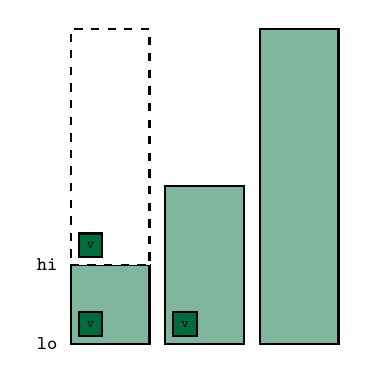
\begin{tikzpicture}
\node at (-0.3,0) {\scriptsize \texttt{lo}};
\node at (-0.3,1) {\scriptsize \texttt{hi}};

% drawing the gens
\draw [fill=mypink, thick] 
  (0,0) -- (1,0) -- (1,1) -- (0,1) -- cycle;
            \draw [fill=mypink, thick] 
  (1.2,0) -- (2.2,0) -- (2.2,2) -- (1.2,2) -- cycle;
            \draw [fill=mypink, thick] 
  (2.4,0) -- (3.4,0) -- (3.4,4) -- (2.4,4) -- cycle;

% drawing the extra malloc portion of from space
\draw<3> [fill=white, dashed, thick] 
  (0,1) -- (1,1) -- (1,4) -- (0,4) -- cycle;

% drawing v in different places
\uncover<2>{\draw [fill=myred, thick]
  (0.1,0.1) -- (0.4,0.1) -- (0.4,0.4) -- (0.1,0.4) -- cycle;
  \node at (0.25,0.25){\tiny \texttt{v}};}
\uncover<3>{\draw [fill=myred, thick]
  (0.1,1.1) -- (0.4,1.1) -- (0.4,1.4) -- (0.1,1.4) -- cycle;
  \node at (0.25,1.25){\tiny \texttt{v}};}
\uncover<4->{\draw [fill=myred, thick]
  (1.3,0.1) -- (1.6,0.1) -- (1.6,0.4) -- (1.3,0.4) -- cycle;
  \node at (1.45,0.25){\tiny \texttt{v}};}
\end{tikzpicture}
\end{center}

\uncover<5>{
Resolved using CompCert's \texttt{extcall\_properties}}
    \end{frame}

\begin{frame}[fragile]{Undefined behavior in C}  
A classic OCaml trick to disambiguate int/ptr:
    \begin{Verbatim}
int test_int_or_ptr (value x) {
    return (int)(((intnat)x)&1); }
    \end{Verbatim}

\uncover<2->{Essentially, assume that pointers are even-aligned.}
\pause \pause

\bigskip

Consider:
\begin{Verbatim}
void foo() {
  char a; char b; char* pa = &a; char* pb = &b;
  if ((pa&1 == 0) && (pb&1 == 0)) { /* elided */ } }
\end{Verbatim}

\pause
True in C, false in exec!

\bigskip

\pause Discussing \texttt{char} alignment issues with CompCert
\end{frame}



\begin{frame}{Reusability: separation between pure and spatial reasoning}
  \centering
  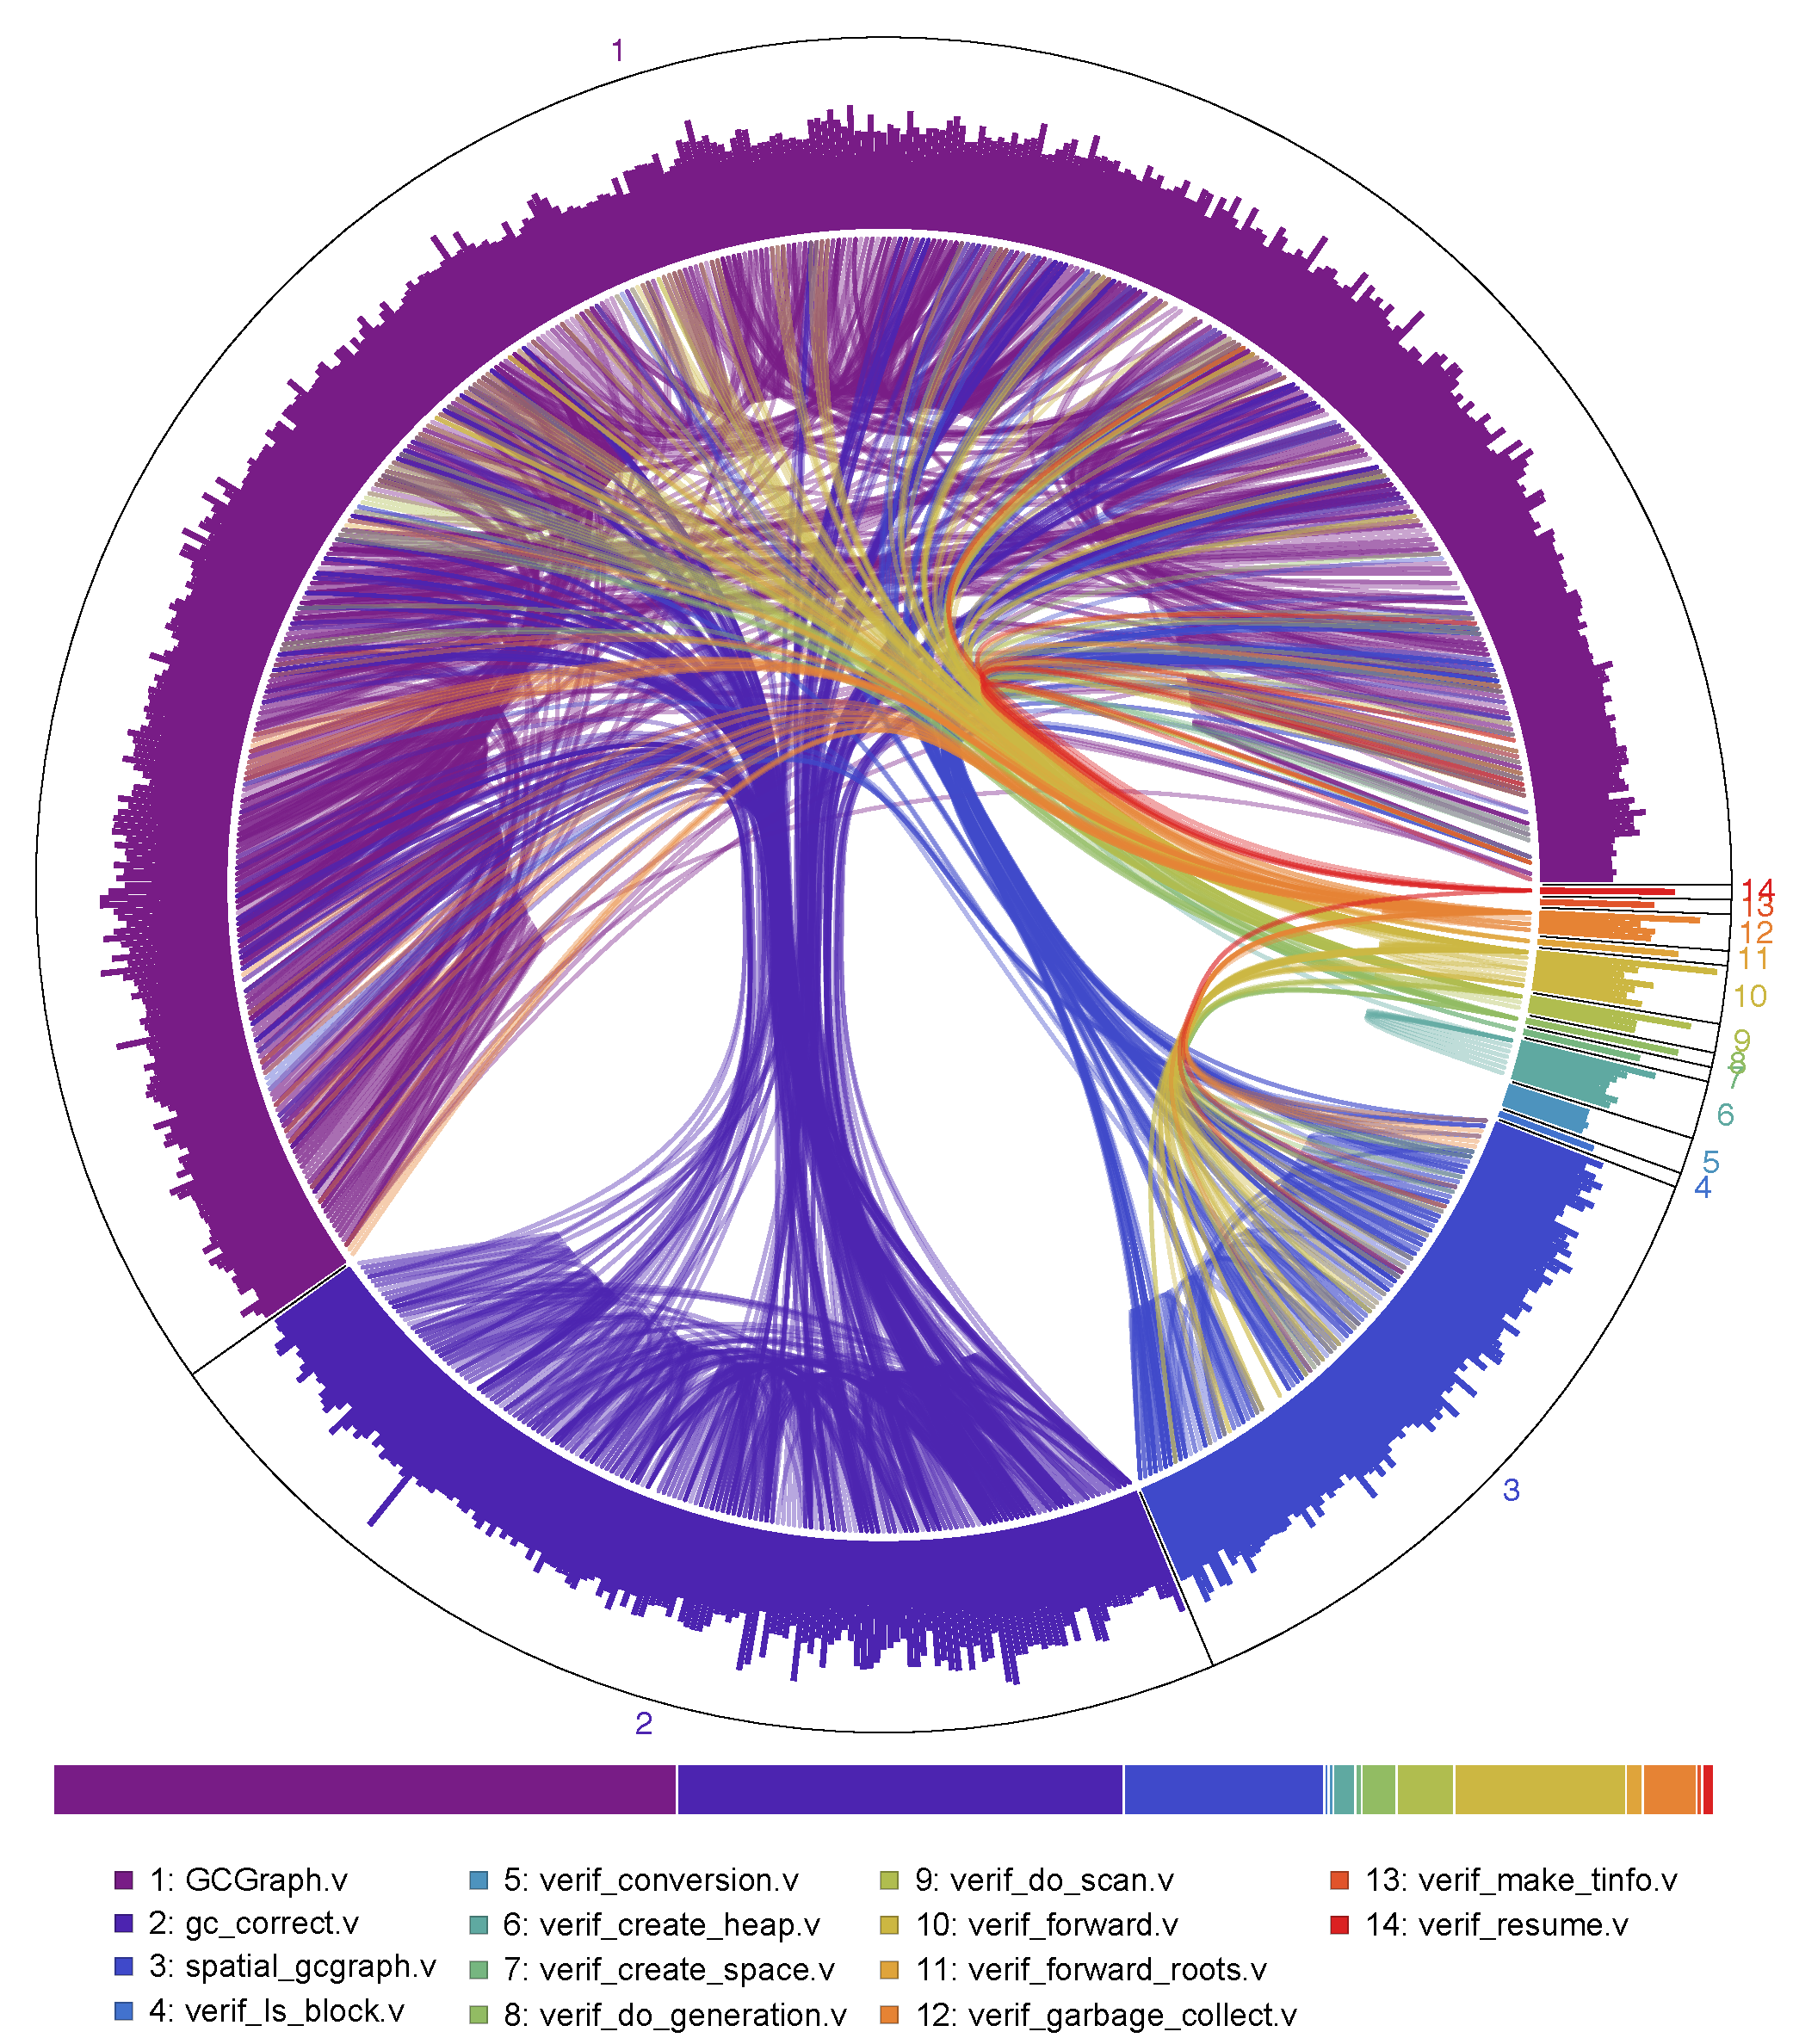
\includegraphics[width=0.9\textwidth]{certigc_theorems.pdf}
\end{frame}

\section{Future Work}
\begin{frame}{Future Work}
  Problems of a \alert{similar shape} \\
  \pause 
  \hspace{1em}serialization \\ 
  \hspace{1em}other collectors

  \bigskip

  \pause
  Towards a verified GC for \alert{OCaml} \\
  \pause 
  \hspace{1em}mutability \\ 
  \hspace{1em}calculate root set \\ 
  \hspace{1em}allow other datatypes

  \bigskip
  \pause \alert{Further refinements} required in C semantics \\ 
  \hspace{1em}before we can \alert{specify} and \alert{verify} OCaml's GC?
  \end{frame}

}
\end{document}
